% Created 2017-11-19 Sun 11:29
\documentclass[11pt]{article}
\usepackage[utf8]{inputenc}
\usepackage[T1]{fontenc}
\usepackage{fixltx2e}
\usepackage{graphicx}
\usepackage{longtable}
\usepackage{float}
\usepackage{wrapfig}
\usepackage{rotating}
\usepackage[normalem]{ulem}
\usepackage{amsmath}
\usepackage{textcomp}
\usepackage{marvosym}
\usepackage{wasysym}
\usepackage{amssymb}
\usepackage{hyperref}
\tolerance=1000
\usepackage[margin=2.5cm]{geometry}
\author{Mathieu Mandret}
\date{}
\title{Algorithme génétique: application au problème du voyageur de commerce.}
\hypersetup{
  pdfkeywords={},
  pdfsubject={},
  pdfcreator={Emacs 25.3.2 (Org mode 8.2.10)}}
\begin{document}

\maketitle
\tableofcontents



\section{Introduction}
\label{sec-1}
\subsection{Le problème du voyageur de commerce}
\label{sec-1-1}
On énonce la situation suivante:
Un commerçant doit se rendre dans une liste de villes données. Il doit passer une seule fois par chaque ville
et revenir à sa ville de départ à la fin de son voyage.
On veut pouvoir savoir dans quel ordre il doit visiter les villes pour parcourir le moins de distance possible.
Mais il se pose un problème d'explosion combinatoire, en effet, pour $n$ villes, il existe $n!$ ordres de parcours.

\emph{Quelques exemples:} \\
Pour $n = 10$ on a $n! = 3628800$, donc pour un parcours contenant 10 villes, il existe plus de 3 millions de parcours possibles.

Pour $n = 30$ on a $n! \simeq 2.65 \times 10^{32}$

Une approche déterministe n'est donc pas envisageable, il faudrait générer toutes ces permutations puis les évaluer unes
par une pour trouver la meilleure ce qui prendrait un temps considérable. 

On observe que la fonction $f: x \rightarrow x!$ croît extrêmement vite:

\begin{figure}[htb]
\centering
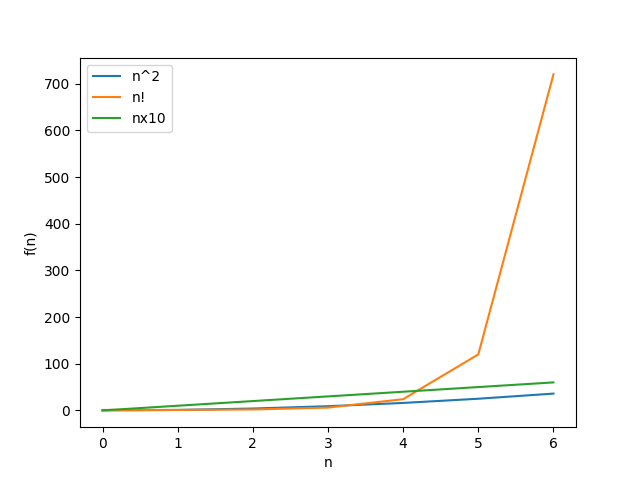
\includegraphics[width=.9\linewidth]{./complexite.png}
\caption{Croissance des fonctions $n^2, n*10$ et $n!$}
\end{figure}

\subsection{Les algorithme génétiques}
\label{sec-1-2}

On peut toutefois espérer trouver une solution approchée à ce problème avec un algorithme génétique.

C'est un type d'algorithme évolutionniste dont le but est de trouver une solution approchée à un problème d'optimisation.
L'algorithme génétique est inspiré de la théorie de l'évolution qui dit que:
\begin{itemize}
\item Une espèce connaitra forcémment des variations aléatoires
\item Si la variation est génante pour l'individu, il ne se reproduira pas ou peu, et cette variation disparaitra
\item Si cette variation est avantageuse, il se reproduira plus et elle se diffusera dans les générations futures.
\end{itemize}

Dans un algorithme génétique, on retrouve toujours les composantes suivantes:

\subsubsection{L'individu}
\label{sec-1-2-1}

C'est simplement une solution potentielle au problème.

\subsubsection{La population}
\label{sec-1-2-2}

Une population est un ensemble d'individus divers. Analogiquement à la biologie, c'est une espèce.    

\subsubsection{La "fitness"}
\label{sec-1-2-3}

C'est une valeur associée à chaque individu, elle permet de quantifier à quel point
une solution est adaptée au problème.
Et des opérations permettant de faire évoluer une population vers une génération meilleure:

\subsubsection{L'évaluation}
\label{sec-1-2-4}

Elle consiste à analyser tous les individus de la population pour associer à chacun une valeur de fitness.

\subsubsection{La séléction}
\label{sec-1-2-5}

C'est la méthode qui permet de choisir dans la population 2 parents pour générer un individu fils.
Si on fait le parallèle avec la théorie de l'évolution, cette opération représente la selection naturelle,
les individus avec les meilleures caractéristiques, et donc la meilleure fitness, on plus de chance de survivre,
ce qui est matérialisé par le fait qu'ils ont plus de chance d'être séléctionnés pour se reproduire et transmettre
leurs caractéristiques au générations futures.

\subsubsection{Le croisement, ou "crossover"}
\label{sec-1-2-6}

Croiser 2 individus représente le processus de reproduction dans la nature. Il revient à créer un individu fils
en combinant 2 parents, les caractéristiques du fils seront alors un mélange aléatoire de celles des parents.

\subsubsection{La mutation}
\label{sec-1-2-7}

Un mutation est un changement aléatoire des caractéristiques d'un individu. 

Pour générer une solution approchée, un algorithme génétique suit le déroulement suivant:

\begin{enumerate}
\item On génère une population d'individus.
\item On les évalue
\item On selectionne les meilleurs individus qui seront les parents de la prochaine génération
\item On les croise pour créer les individus fils
\item On fait muter une partie de ces fils
\end{enumerate}

On peut ensuite répéter ces étapes autant de fois qu'on le souhaite, jusqu'a obtenir un résultat satisfaisant,
il faut alors une condition d'arrêt, qui peut être par exemple une valeur de fitness cible ou un nombre limite de générations.
On peut modéliser ce déroulement avec un diagramme:
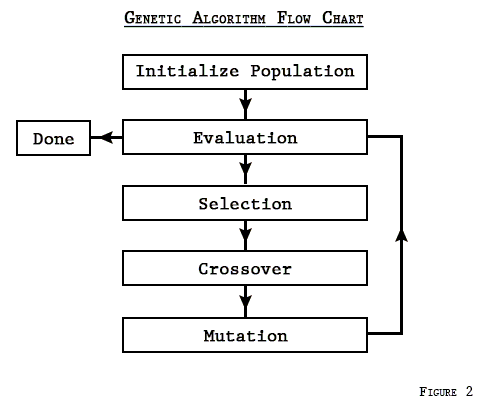
\includegraphics[width=.5\linewidth]{./GA.png}
\end{document}
